\documentclass[a4paper, 12pt, oneside]{scrartcl}
%\documentclass[a4paper, 12pt, oneside]{ncc}
\usepackage[warn]{mathtext}          % русские буквы в формулах, с предупреждением
\usepackage[T2A]{fontenc}            % внутренняя кодировка  TeX
\usepackage[utf8]{inputenc}         % кодовая страница документа
\usepackage[english, russian]{babel} % локализация и переносы
\usepackage{indentfirst}   % русский стиль: отступ первого абзаца раздела
\usepackage{misccorr}      % точка в номерах заголовков
\usepackage{cmap}          % русский поиск в pdf
\usepackage{graphicx}      % Работа с графикой \includegraphics{
\graphicspath{{transform/}}
\usepackage{psfrag}        % Замена тагов на eps картинкаx
\usepackage{caption2}      % Работа с подписями для фигур, таблиц и пр.
\usepackage{soul}          % Разряженный текст \so{ и подчеркивание \ul{
\usepackage{soulutf8}      % Поддержка UTF8 в soul
\usepackage{fancyhdr}      % Для работы с колонтитулами
\usepackage{multirow}      % Аналог multicolumn для строк
\usepackage{ltxtable}      % Микс tabularx и longtable
\usepackage{paralist}      % Списки с отступом только в первой строчке
%\usepackage{longtable}
%\usepackage{tabularx}
\usepackage[perpage]{footmisc} % Нумерация сносок на каждой странице с 1
\usepackage{amsmath}
\usepackage{amsfonts}
\usepackage{amssymb}
\usepackage{tabularx}  %продвинутые таблицы
\usepackage{fancyhdr} %колонтитулы
\usepackage{longtable}
\usepackage[table]{xcolor} %цвета ячеек
% Задаем отступы: слева 30 мм, справа 10 мм, сверху до колонтитула 10 мм
% снизу 25 мм
%\usepackage[a4paper, top=10mm, left=30mm, right=10mm, bottom=25mm]{geometry}
% Нумерация формул, картинок и таблиц по секциям
\numberwithin{equation}{section}
\numberwithin{table}{section}
\numberwithin{figure}{section}
% % % % % % % % % % % % % % % % % % % % % % % % % % % % % % % % % % % % % % % %
% % % % %
\begin{document}
\section*{Пункт -1}
В данном отчете все скрипты написаны с использованием языка python3.6 и следующих фрэймфорков, упрощающих рутину: numpy, 
scikit-learn, pandas, seaborn, os, matplotlib. Работа со всеми случайностями в перемешивании, разбиении и инициализации 
возлагается на scikit-learn и его встроенные опции для контроля случайных чисел, такие как random state. В качестве метрики качества 
используется $ R^2 $, так как она позволяет сравнить между собой две модели в разных масштабах и при нелинейных преобразованих.
(Примечание: некоторые переменные и названия графиков сохранили в себе RSS, так как первоначально использовалась именно 
    эта метрика, которая впоследствии была заменена на $ R^2 $ в связи с несравнимостью некоторых моделей по среднеквадратичной 
ошибке. Если где-то я случайно пропустил mean squared error в подписи к графикам, то там имеется в виду $ R^2 $)

\section*{Пункт 0}
Сначала нарисуем попарные диаграммы рассеивания с гистограммами на диагонали. Рисунок слишком большой, чтобы вставлять его в отчет, потому
см. вложенный в архив файл sm.png. Рассмотрим сначала диаграммы рассеяния предикторов и целевой переменной: налицо достаточно сильные 
положительные корреляции целевой переменной и признаков Beds, Baths, Square feet. Ожидаем, что эти признаки внесут в объясненную 
вариацию целевой переменной значительную часть и войдут в уравнение регрессии с положительными коэффициентами. Кроме того, 
заметим, что имеется также чуть менее выраженная отрицательная корреляция целевой переменной с ковариатами Miles to resort, Miles to base.
Далее следует практически полное отсутствие корреляции зависимой переменной с регрессором Acres, слабая положительная корреляция с Cars и
предположительно нелинейная связь с Years old, возможно данная зависимость является квадратичной. Теперь рассмотрим связь предикторов между 
собой: видим, что Beds достаточно сильно положительно коррелирует с Baths и Square feet, следовательно среди регрессоров наблюдается 
явление мультиколлинеарности, которое может скрыть истинные зависимости, поэтому без регуляризации не обойтись. Далее Square feet 
коррелирует с Baths, Miles to resort с Miles to base. В остальном диаграммы рассеяния выглядят либо случайно, либо прослеживается 
некоторая нелинейная связь, которая не должна влиять на модель. На некоторых диаграммах можно заметить выбросы (особенно это заметно 
на гистограмме Years old, Acres)
(правильнее будет сказать influential observations, наверное), которые могут 
вносить шум в модель. \\
В последнюю очередь заметим, что некоторые гистограммы выглядят асимметрично или имеют тяжелые хвосты, а значит взятие логарифма может 
потенциально улучшить результаты, поскольку регрессия хорошо предсказывает те наблюдения, которые близки к средним. Так же можно попробовать 
добавить $$ Years\_old^2  $$ в модель.

\section*{Пункт 1}
Для разбиения выборки псевдослучайным образом на обучающую и тестовую воспользуемся встроенной в scikit-learn рутиной из модуля model selection: 
train test split. Зададим seed и необходимые пропорции. Подробности в скрипте main.py.

\section*{Пункт 2}
Очевидно, что параметры lasso регрессии будут быстрее сходиться к нулю с увеличением коэффициента регуляризации, чем параметры ridge регрессии, 
поэтому зададим для lasso регрессии диапазон вариации коэффициента меньше, чем для ridge регрессии: 0-150 и 0-300 соответственно. Стандартизуем 
обучающую и тестовую выборки. Нанесем на график линии $ R^2 $ для оптимального константного прогноза, коим является среднее значение 
целевой переменной. Построим 
для каждого выбранного коэффициента регуляризации модель соответствующей регресии. Ниже изображены графики зависимостей метрики $ R^2 $ 
от коэффициента регуляризации по сравнению с оптимальным константным прогнозом.
\begin{figure}[h]
    \centering
    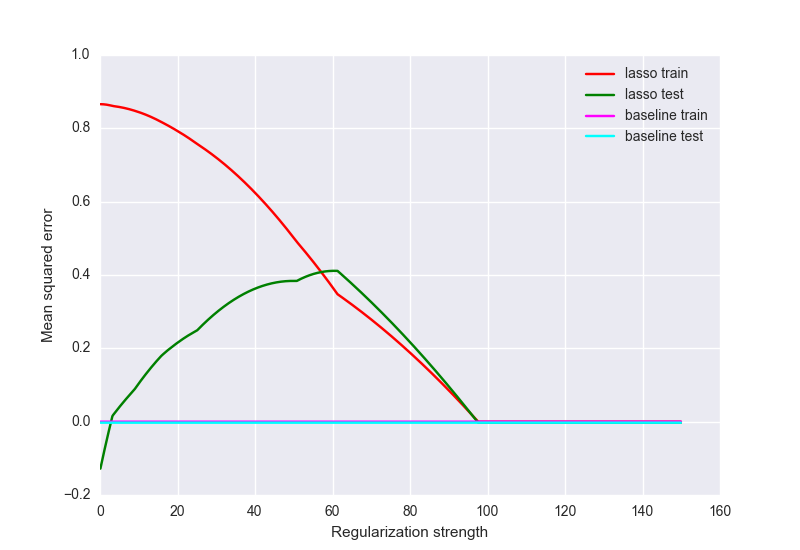
\includegraphics[width=\linewidth]{rss_lasso.png}
\end{figure}
\newline
\begin{figure}[h]
    \centering
    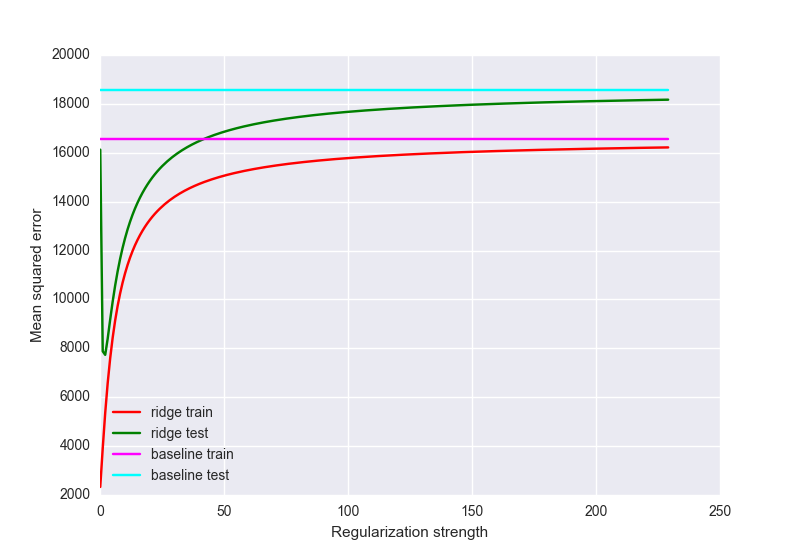
\includegraphics[width=\linewidth]{rss_ridge.png}
\end{figure}

\newpage
Видно, что для обучающих выборок метрика всюду больше, чем для регрессии на константу, и только при очень сильной регуляризации эта метрика сходится 
к эр квадрат константного прогноза, причем для lasso регрессии намного быстрее, чем для ridge регрессии. С другой стороны, на тестовых данных модель сначала 
показывает себя хуже, чем константная, но с увеличением коэффициента регуляризации начинает показывать хорошие значения, после чего сходится к константному прогнозу.

\section*{Пункт 3}
Построим графики зависимости коэффициентом линейной регрессии от коэффициента регуляризации. Ниже представлены графики.
\begin{figure}[H]
    \centering
    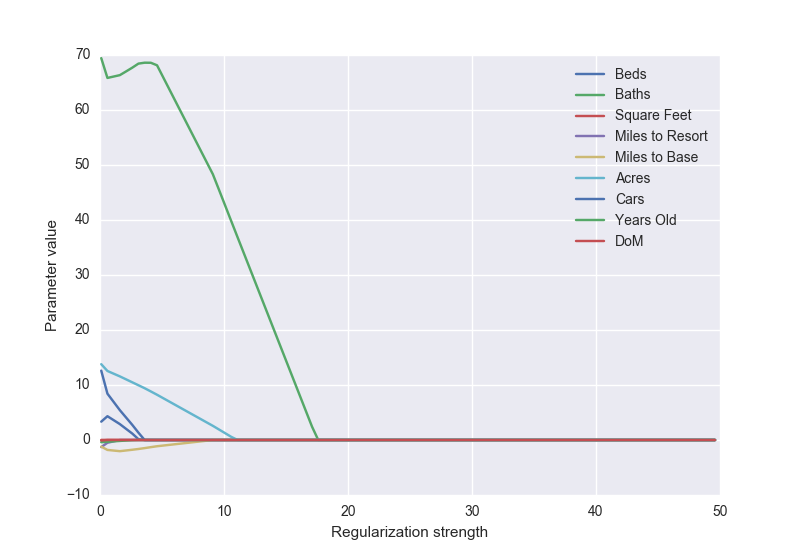
\includegraphics[width=\linewidth]{Lasso_params.png}
\end{figure}

\begin{figure}[H]
    \centering
    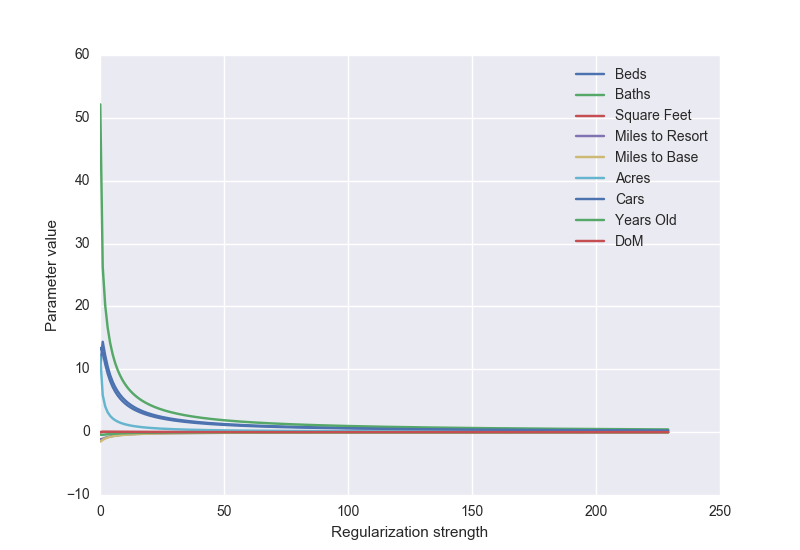
\includegraphics[width=\linewidth]{Ridge_params.png}
\end{figure}

\newpage
\section*{Пункт 4}
Согласно графикам выше в лассо регрессии последними в ноль сваливаются признаки Baths, Acres, в ридж регрессии Baths, Square feet. Будем считать их 
наиболее значимыми. Оптимальным методом по результатам теста оказалась модель ridge регрессии с коэффиицентом регуляризации 50.1 c $ R^2 $ 
0.58, что можно наблюдать на графиках из пункта 3. Значения коэффициентов сохранены в файл results.txt, вложенный в архив с отчетом. 

\section*{Пункт 5}
Построим еще несколько моделей на 4 разных “сидах”. С результатами работы кода, кодом
и графиками можно ознакомиться в папке seed, вложенной в архив с отчетом. В целом выводы 
такие: качество модели и параметры достаточно сильно зависят от разбиения выборки на 
обучающие и тестовые множества, регрессия оказалась чувствительной к вариации данных. 
Значения параметров “прыгают” в пределах 10-20 единиц. Среди 
этих моделей нашлась более удачная в терминах $ R^2 $, 
чем найденная в в предыдущих пунктах. Это ridge регрессия с параметром регуляризации = 4.1.
Ее коэффициенты в порядке перечисления регрессоров в таблице данных к заданию: 
[ 12.45281427  39.09180782  23.08333275 -26.9412894  -24.96807001
27.09034573   9.31500178  -9.16824244   5.4078637 ].

\section*{Пункт 6}
Построим модель с выбранным значением гиперпараметра (50.1 из первых пунктов) теперь уже на полной выборке. 
Далее проведем ее тест, разбив с изначальным “сидом” на обучающее и тестовое множества аналогично 
пункту 1. Результаты работы следующие. Коэффициенты в порядке перечисления в таблице: 
[19.001, 25.091, 20.8, -14.968, -18.168, 8.839, 12.186, -7.776, 7.5], $ R^2 $ = 0.82
Наблюдаем не очень значительные изменения в параметрах модели, но именно это и ожидалось, 
так как мы добавили информации в данные, построив модель на полной выборке. Видим так же, что 
на тестовом подмножестве исходной выборки $ R^2 $ оказывается значительно выше. 
Скрипт с кодом содержится в папке full, вложенной в архив с отчетом.

\section*{Пункт 7}
В пункте 0 высказывалось предположение, что логарифмирование может потенциально улучшить предиктивную 
силу регрессии. Проверим это, взяв log(x + 1) от целевой переменной и ряда предикторов: Miles to resort, 
Miles to base, square feet, Acres, Years old, dom. Разобьем выборку с тем же “сидом”, что и в первых 
пунктах, чтобы можно было сравнить результаты. Повторим все в точности так же, как делали в первых пунктах.
Ниже представлены графики полученных результатов.
\begin{figure}[H]
    \centering
    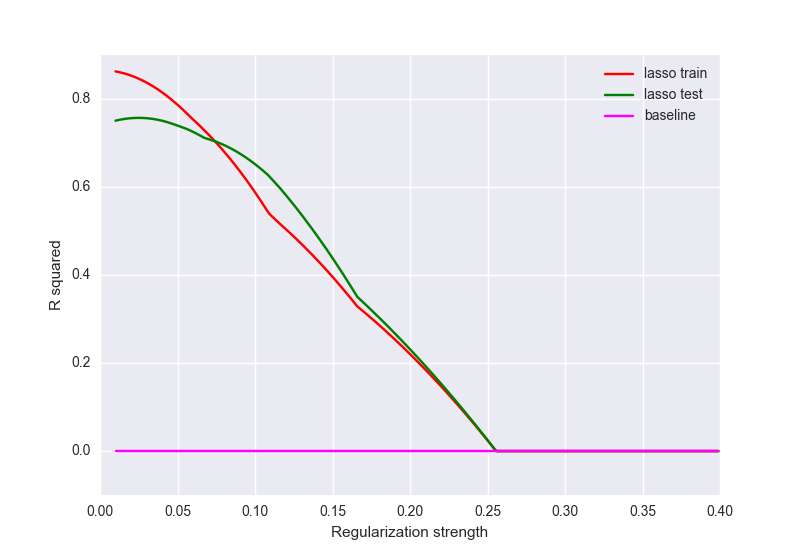
\includegraphics[width=\linewidth]{r2_lasso.png}
\end{figure}

\begin{figure}[H]
    \centering
    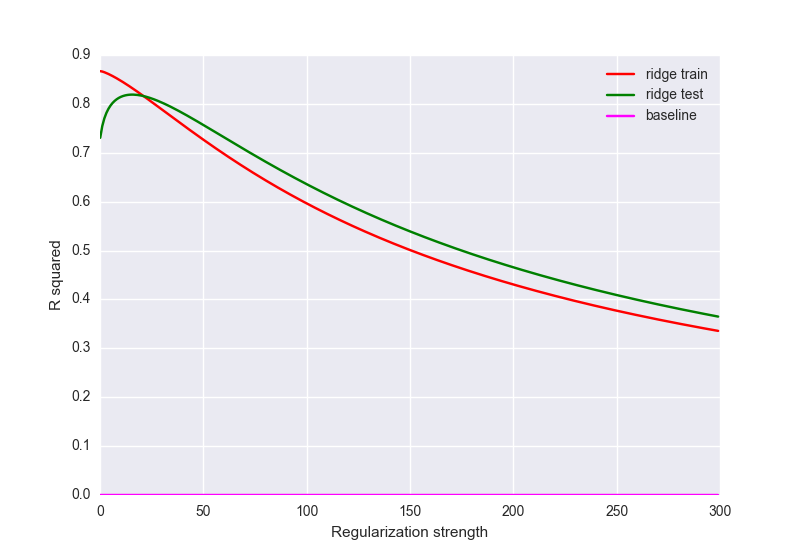
\includegraphics[width=\linewidth]{r2_ridge.png}
\end{figure}
\newpage
\begin{figure}
    \centering
    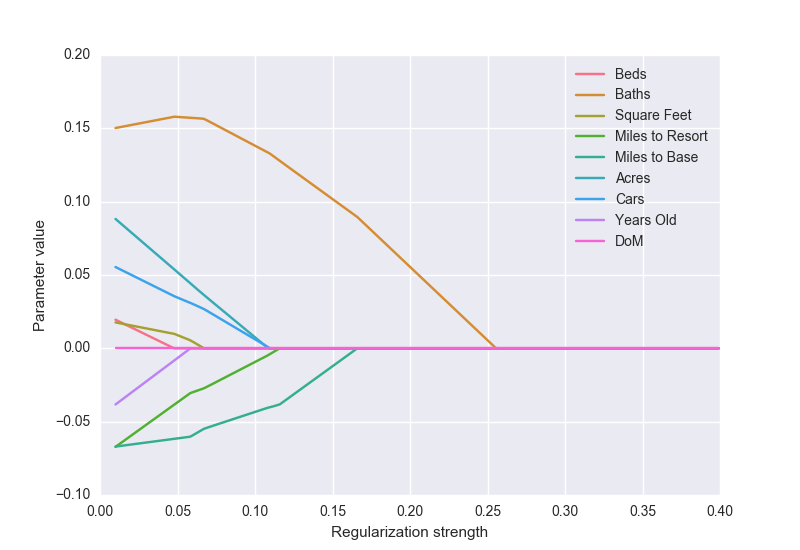
\includegraphics[width=\linewidth]{lasso__params.png}
\end{figure}

\begin{figure}
    \centering
    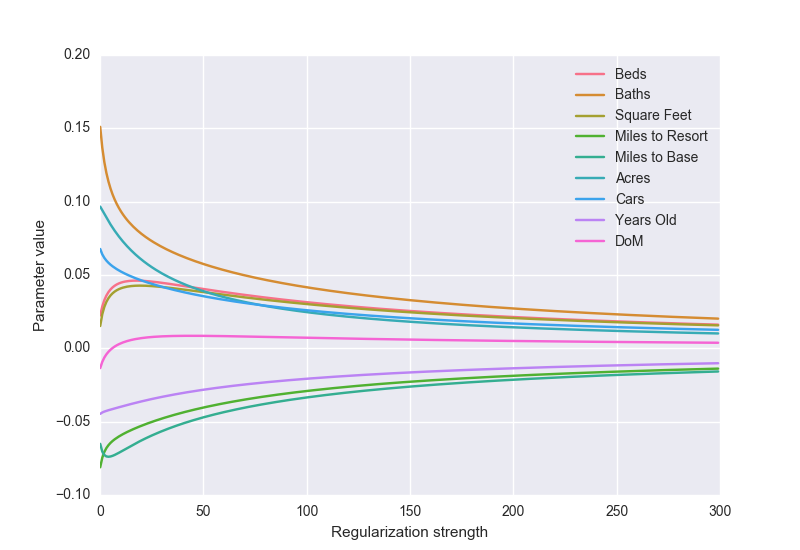
\includegraphics[width=\linewidth]{ridge__params.png}
\end{figure}

Видно, что логарифмическое преобразование переменных привело к улучшению качества 
моделей в терминах метрики $ R^2 $, в частности в ridge регресии произошел скачок с 
0.5 до 0.8, а значит трансформированные переменные дают больший вклад в вариацию целевой переменной, 
чем изначальные предикторы. Скрипт с кодом находится в папке transform, вложенной в архив с отчетом.

\end{document}
